\documentclass[]{beamer}
\usepackage{color}
\usepackage{listings}
\usepackage{verbatim}
\usepackage{graphicx}
\usepackage{multicol}
\usepackage[utf8]{inputenc}
\usepackage{amsmath}
\usepackage{graphicx}
\usetheme{Madrid}
\title{Bachelor-Thesis Proposal}
\subtitle{Simulation of the RoboCup Logistic League with Fawkes and Gazebo for Multi-Robot Coordination Evaluation}
\author {Frederik Zwilling}
\institute{RWTH Aachen}
\date{23.07.2013}
\subject{Multi-Robot Simulation}

\begin{document}
\frame{\titlepage}

%Übersicht
%\begin{frame}
%\frametitle{Overview}
%\begin{enumerate}
%\item Motivation
%\item Software Foundation
%\item Goals
%\item Conclusion
%\end{enumerate}
%\end{frame}

%Motivation
\begin{frame}
\frametitle{Motivation}
\begin{multicols}{2}
\begin{figure}
\only<1>{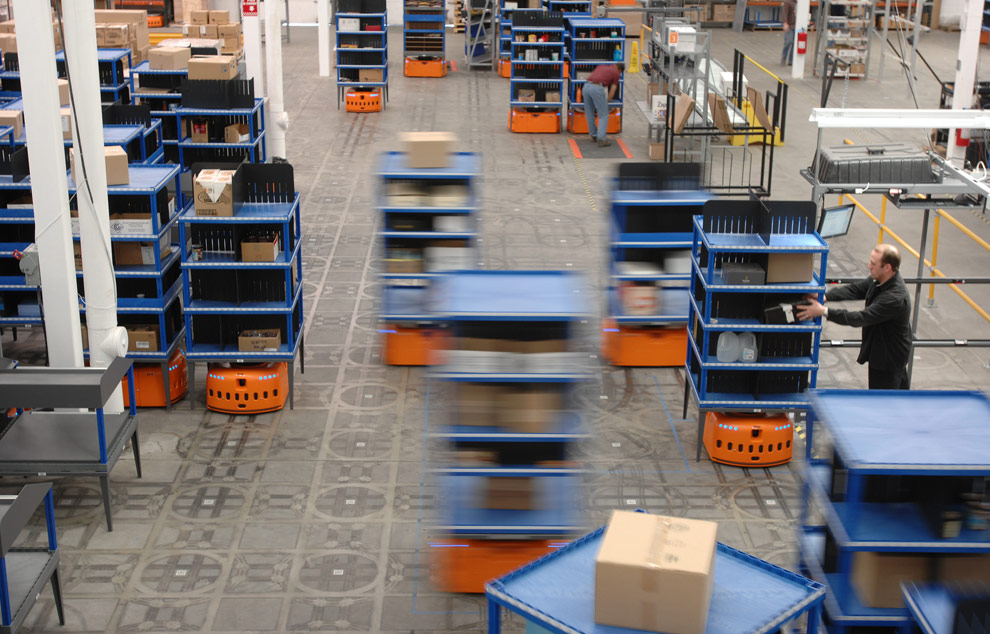
\includegraphics[width=140pt]{pics/kiva.jpg}\\}
\only<2>{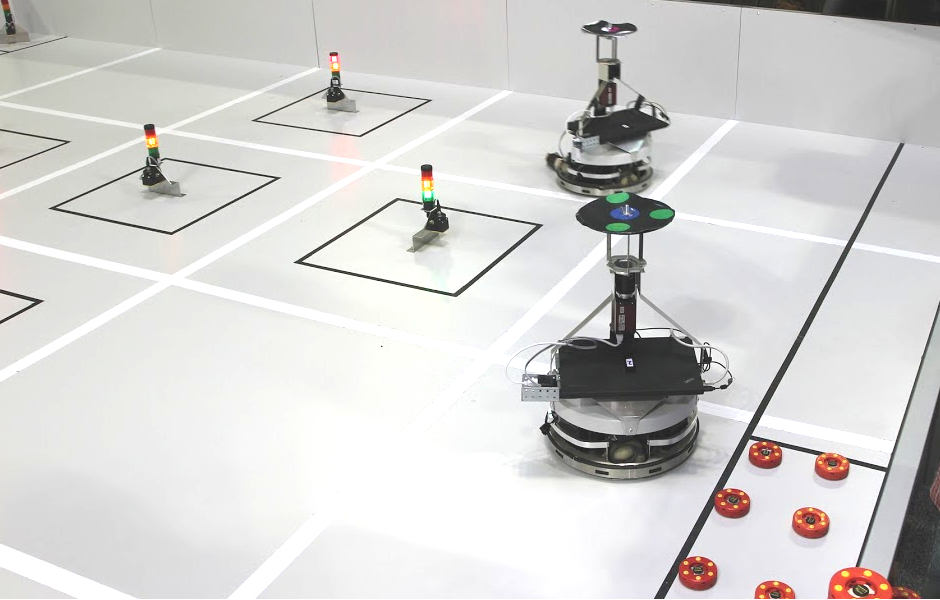
\includegraphics[width=140pt]{pics/llsf.jpg}\\}
\only<3->{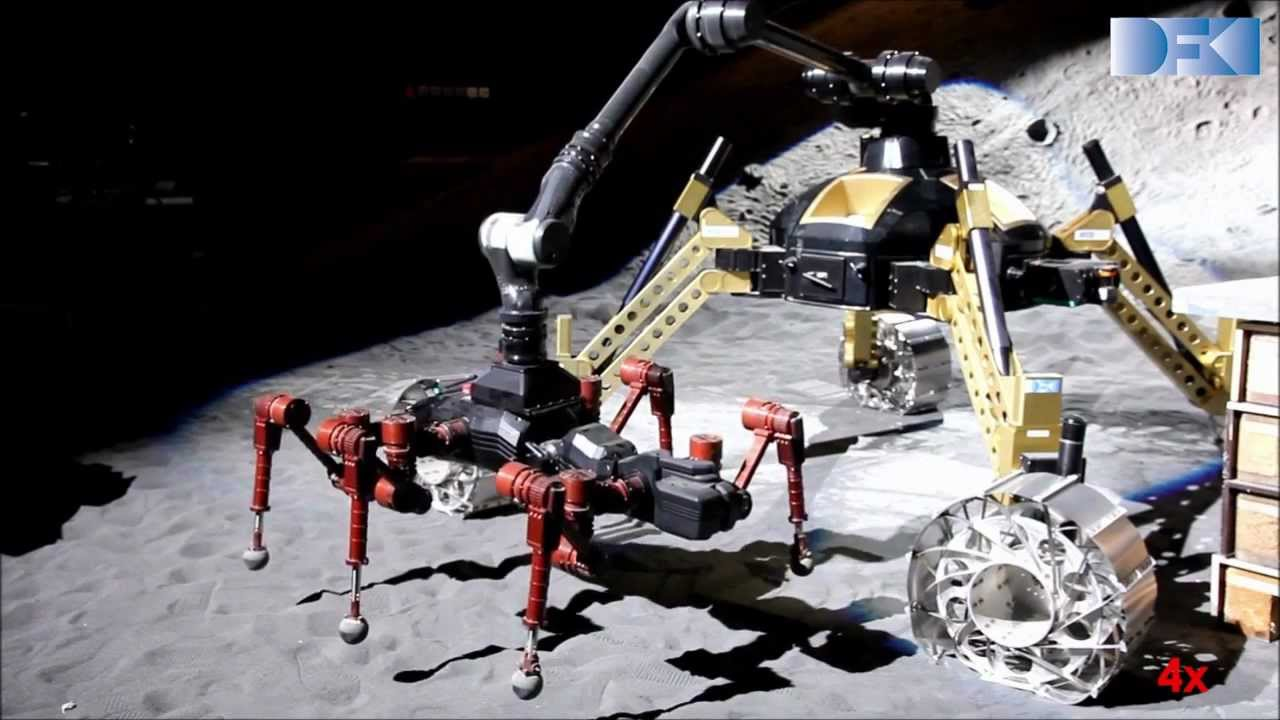
\includegraphics[width=140pt]{pics/rimes.jpg}\\}
\end{figure}
Fields with multi-robot systems:
\begin{itemize}
\item<1-> warehousing
\item<2-> logistics
\item<3-> space exploration
\end{itemize}
\end{multicols}
\pause \pause \pause 
\begin{itemize}
\item[$\Rightarrow$] Multi-robot systems are useful and about to become more important
\end{itemize}
\end{frame}

\begin{frame}
\frametitle{Logistic League sponsored by Festo (LLSF)}
\fboxsep=0pt
\noindent%
\begin{minipage}[]{0.48\linewidth}
\begin{figure}
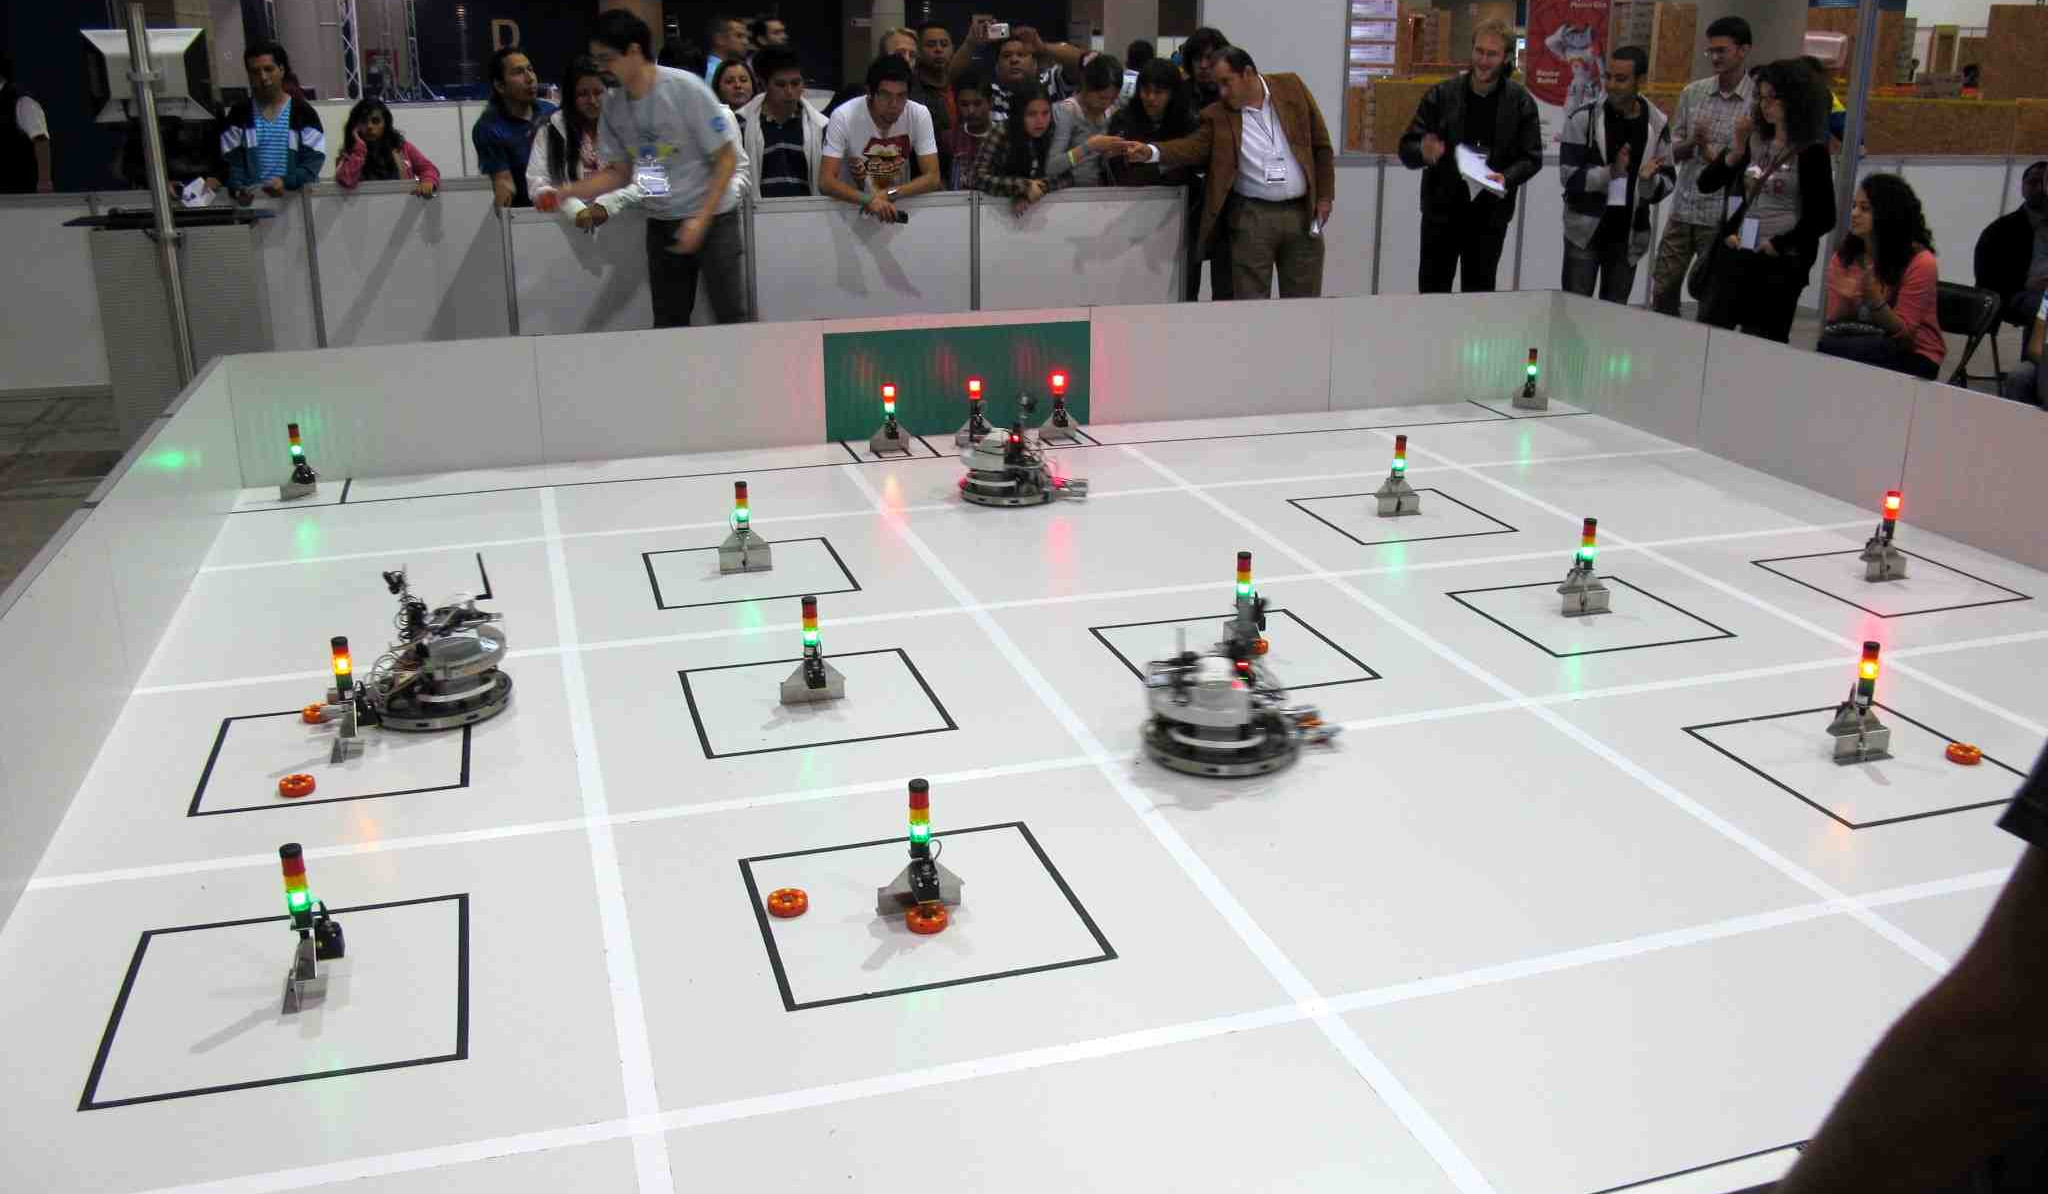
\includegraphics[width=150pt,heigth=120pt]{pics/llsfLeague.png}\\
\end{figure}
\end{minipage}%
\hfill%
\begin{minipage}[]{0.48\linewidth}
League:
\begin{itemize}
\item Part of RoboCup competition
\item Testbed for logistic robots in a competitive factory automation scenario
\end{itemize}
\pause
Task:
\begin{itemize}
\item Produce and deliver products by feeding machines% with resources and semi-finished products
\item Optimize workflow and performance of the system
\item Being robust against failure
\end{itemize}
\end{minipage}
\end{frame}

\begin{frame}
\frametitle{Problem-Solution}
\begin{multicols}{2}
Testing Problems:
\begin{itemize}
\item Need for environment and robots 
\item Setup of the robots  %Effort scaleing with number of robots
\item Separate testing of high level components
%\item Effort scaling with the number of robots
\item Time-consuming comparison of multi-agent strategies
\pause
\item[$\Rightarrow$] Testing is time and resource consuming
\end{itemize}
\pause
Advantages of a Simulator:
\begin{itemize}
\item Simulated environment and robots
\item Only setup of the software
\item Providing ground truth simulation
%\item Adding more robots more easily in the simulation
\item Simulation running over night or in parallel
\pause
\item[$\Rightarrow$] Simulation saves time and resources
\end{itemize}
\end{multicols}
\pause
\begin{block}{Thesis Topic}
Developing a multi-robot simulation to evaluate multi-agent strategies
\end{block}
\end{frame}

\begin{frame}
\frametitle{Gazebo}
\begin{multicols}{2}
An Open Source robot simulator
\begin{figure}
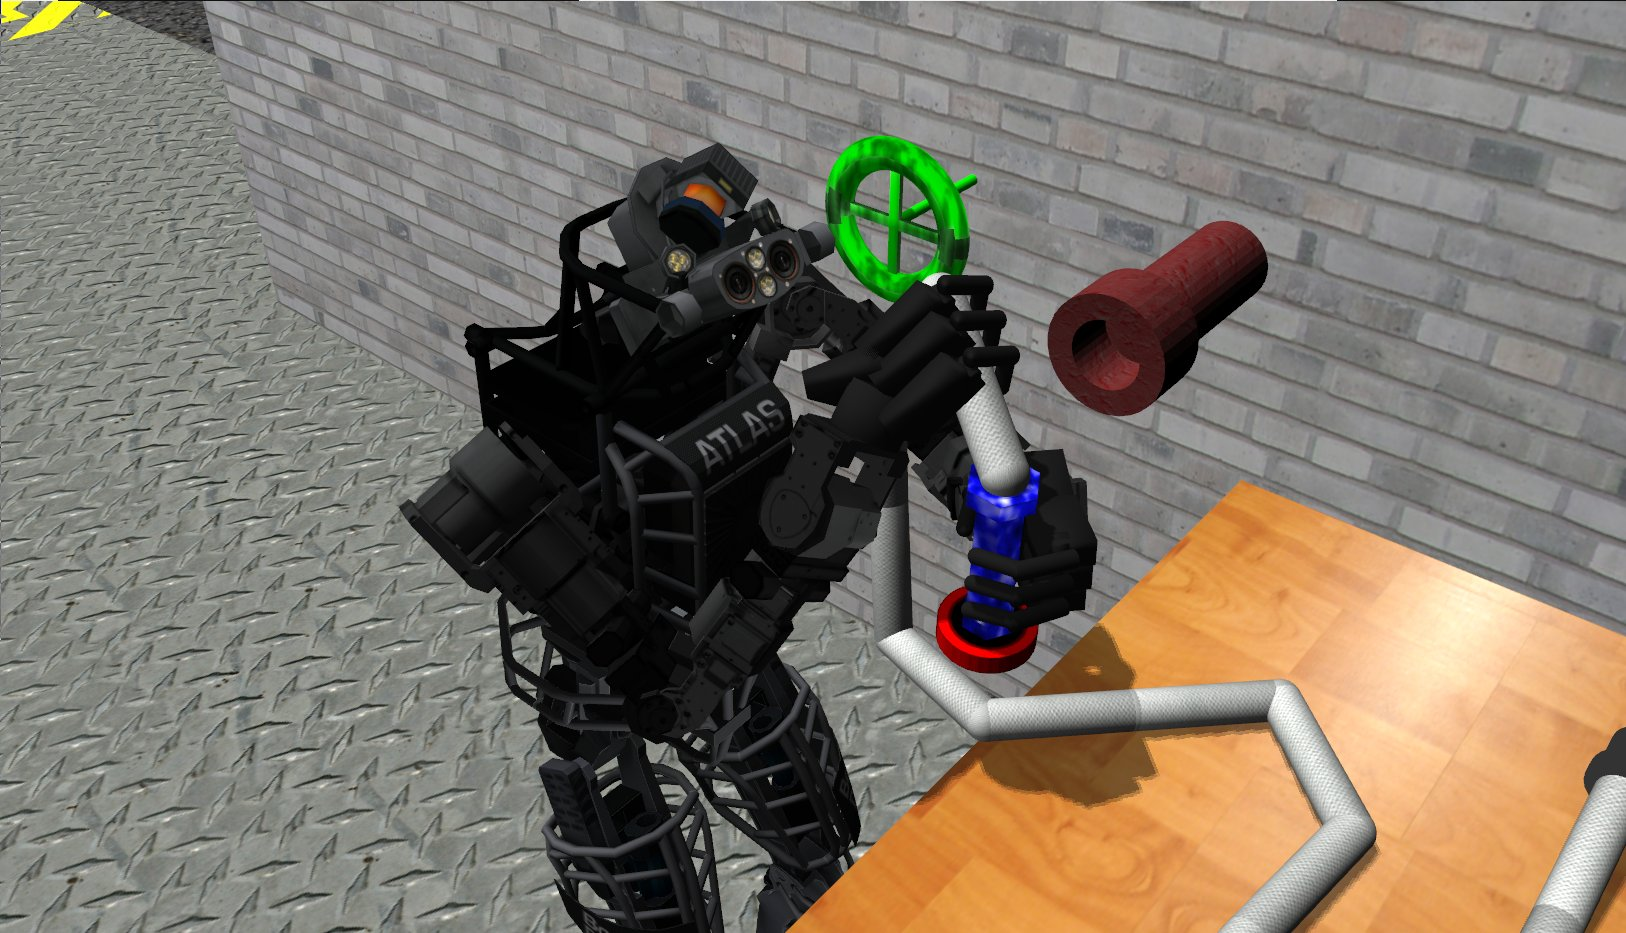
\includegraphics[scale=0.13]{pics/gazebo.jpg}
\end{figure}
\begin{itemize}
\item Powerful graphics and physics engines %Reflections, Slippery (Odom)
\item Already supports some robots and sensors (e.g. Hokuyo laser sensor)
\item Related work with Gazebo (Scene Reconstruction, Multi-Level Abstraction)
\item Extensive support
\end{itemize}
\end{multicols}
\pause
\begin{itemize}
\item[$\Rightarrow$] Suitable simulator for the thesis and future work
\end{itemize}
\end{frame}

\begin{frame}
\frametitle{Fawkes}
\begin{multicols}{2}
\begin{figure}
\only<1>{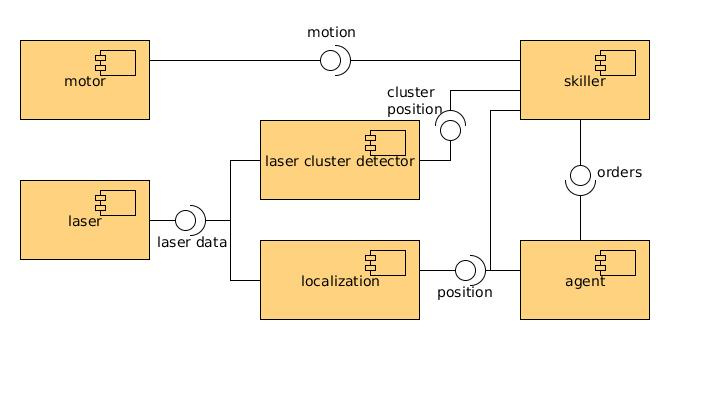
\includegraphics[scale=0.26]{components/simplefawkes.jpg}}
\only<2>{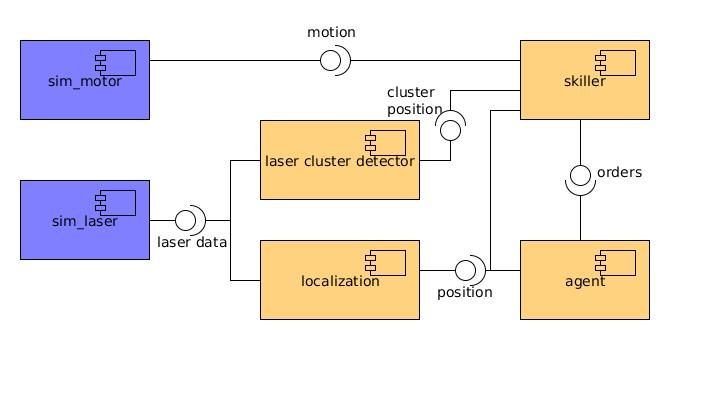
\includegraphics[scale=0.26]{components/lowsim.jpg}}
\only<3>{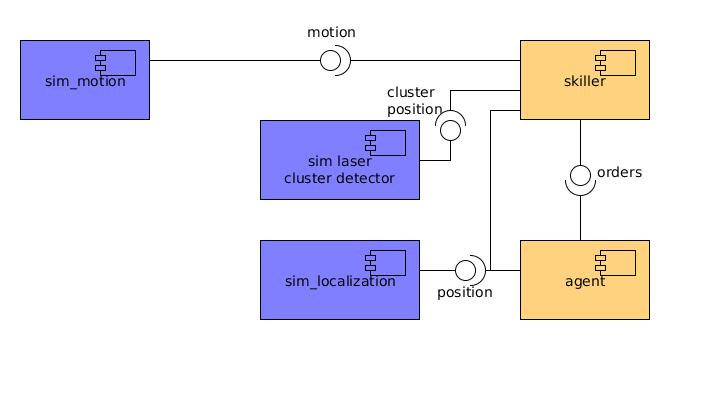
\includegraphics[scale=0.26]{components/highsim.jpg}}
\end{figure}
An Open Source robot software framework
\begin{itemize}
\item Developed and used primarily at KBSG
\item Component-based software design
\item Blackboard communication infrastructure%,\\ plugins communicate through interfaces
\pause
\end{itemize}
\end{multicols}
\begin{itemize}
\item[$\Rightarrow$] Easy exchange of sensor/actuator plugins by simulation plugins
\end{itemize}
\end{frame}

\begin{frame}
\frametitle{Goals of the Thesis}
Simulation of sensors and actuators
\begin{itemize}
\item High level simulation
\item Low level simulation
\end{itemize}
\pause
Simulation environment for LLSF
\begin{itemize}
\item Modeling the reactive environment
%\item Implement machine behavior, rules, ...
\end{itemize}
\pause
Multi-agent simulation
\begin{itemize}
\item Mapping Fawkes instances - simulated robots
%\item Communication between agents
\end{itemize}
\pause
Expandability for future changes/extensions
\begin{itemize}
\item General interfaces between Fawkes and Gazebo
\item Modularity (e.g. exchange webcam with stereo camera)
\end{itemize}
%Multi-level abstraction
%LLSF Challenges
\end{frame}

\begin{frame}
\frametitle{Multi-Agent Strategies, Evaluation}
Comparison of multi-agent strategies
\begin{itemize}
\item Current role-based approach vs. dynamic role allocation
\item Comparing different roles (e.g. production vs. recycling role)
\end{itemize}
\pause
Evaluation
\begin{itemize}
\item Qualitative\\(differences real world - simulation)
\item Quantitative\\(resource usage, scalability)
\end{itemize}
\end{frame}

\begin{frame}
\frametitle{Conclusion}
\begin{itemize}
\item Multi-Robot Systems getting more important
\item Development/testing difficult and time-consuming
\item[$\Rightarrow$] Simulation is a key to efficient development/testing
\pause
\item Goals: 
\begin{itemize}
\item LLSF simulation
\item  high/low level simulation
\item  expandability
\item  comparison of multi-agent strategies
\end{itemize}
\pause
%\item Short presentation of current state of development
\end{itemize}
\end{frame}


\end{document}
